\chapter{Marco teórico: Sistemas de recomendación}\label{chap:recom}




\section{Contexto: El premio Netflix}

Como ejemplo para mostrar la importancia que tienen para las empresas los sistemas de recomendación se va a hacer una presentación de lo que fue el Premio Netflix. Dicho premio fue una competición abierta para generar un algoritmo de filtrado colaborativo para predecir las puntuaciones de películas que darían los usuarios, basándose en puntuaciones anteriores, sin mayor información sobre los usuarios o las películas, esto es, sin saber la película puntuada más allá de su id.\\

La competición fue organizada por Netflix, una compañía que por aquél entonces se dedicaba al alquiler de películas y estaba abierta a cualquier persona no relacionada con Netflix. En su edición del año 2009, contó con un premio de 1 millón de dólares, que fue ganado por el equipo de \textit{BellKor's Pragmatic Chaos} \cite{netflix}, cuyo algoritmo mejoró el  error en las puntuaciones dadas por el algoritmo de Netflix alrededor de un $10 \%$.\\

Netflix proporcionó un dataset de entrenamiento de 100 millones de registros, dados por $480000$ usuarios a un total de $18000$ películas. Cada registro es una $4-$tupla de la forma $(user,\ movie,\ date\ of\ grade,\ grade)$. El usuario y la película son id enteros mientras que las puntuaciones van de $1$ a $5$ (enteros).\\

El dataset de test tenía alrededor de 3 millones de registros, usándose la mitad para determinar a los ganadores y la otra mitad para actualizar las tablas de líderes. Como es norma, las puntuaciones contenidas en este dataset de test únicamente eran conocidas por el jurado, con el fin de evitar un overfitting a los datos de test \cite{overfitting}.\\

Este cuantioso premio tuvo a varios grupos formados por expertos en el terreno durante varios años intentando conseguir el mejor algoritmo posible. Es evidente que un premio de esas características para un algoritmo de filtrado significa que es un área de vital importancia para la empresa organizadora, Netflix.

\section{Introducción}

Los sistemas de recomendación son un tipo de filtros de información, que buscan predecir la puntuación (preferencia) que un usuario daría a un objeto en particular. Su principal uso está relacionado con aplicaciones de uso comercial, lo cual hace que el funcionamiento de los sistemas más avanzados y los datos de entrenamiento disponibles sean limitados.\\

En los últimos años ha habido un crecimiento en el interés de los sistemas de recomendación \cite{Abdomavicius}, desde la aparición de los primeros artículos al respecto a mediados de los años 90 \cite{resnick}. Por ejemplo, en \cite{nageswara} puede encontrarse un inventario de sistemas de recomendación existentes que han sido desarrollados tanto en un ámbito académico como en la industria.\\

Los sistemas de recomendación son utilizados en diversas áreas, muchas veces aplicados como recomendadores de productos en servicios como Amazon, generadores de colas de reproducción en servicios de música y vídeo (Netflix, YouTube, Spotify), o recomendadores de contenido como en el caso de Twitter o la mayoría de veriones digitales de periódicos. Además, hay sistemas de recomendación de tipos menos habituales, como por ejemplo los recomendadores de parejas que pueden encontrarse en aplicaciones como Tinder.\\

En la creación de sistemas de recomendación existen dos corrientes principales e incluso una tercera, derivada de las dos primeras. En este capítulo explicaremos en detalle estas corrientes existentes en el campo de los sistemas de recomendación, con el fin de explicar el marco conceptual del trabajo y justificar las decisiones tomadas a la hora de la creación del mismo. Los tres tipos principales de sistemas de recomendación son los siguientes:

\begin{itemize}
    \item \textbf{Filtrado colaborativo}: Este tipo de filtros utilizan el feedback dado por el usuario y el resto de usuarios en el pasado sobre el conjunto de items, con el fin de poder predecir qué item puede ser valorado positivamente por el usuario. Un ejemplo sería una tienda que utiliza las valoraciones de un usuario concreto y del resto de usuarios para recomendar a ese usuario concreto los productos que predicen serán valorados con la mejor puntuación de entre aquellos que aun no figuran en su historial de compra o puntuación.
    \item \textbf{Filtrado basado en contenido}: Este tipo de filtros utilizan metadatos de los items en cuestión para inferir la relación entre un usuario y esa metainformación. Sería por ejemplo un sistema en una tienda que recomienda items a un usuario pero sin tener en cuenta su feedback, simplemente buscando productos similares (por ejemplo, de la misma sección, rango de precio...)
    \item \textbf{Sistemas híbridos}: Combinan los dos tipos de sistemas de recomendación anteriores, de diferentes formas, con el fin de potenciar sus virtudes y disminuir sus defectos.
\end{itemize}

\section{Marco conceptual. Tipos de sistemas de colaboración.}\label{sec:marcoconceptual}

\subsection{Filtrado colaborativo}

Los sistemas de recomendación basados en filtrado colaborativo, parten de la premisa de que los usuarios que han votado parecido que una persona dada unos items, son relevantes a la hora de definir qué items han de ser recomendados a la persona dada. Además, los items que tienen puntuaciones similares, también son relevantes. Son los tipos de modelos más utilizados por compañías como Amazon \cite{Amazon} o Google \cite{Google}\\

En el filtrado colaborativo, el sistema recoge como entrada un conjunto de puntuaciones de los usuarios sobre una serie de items. Los usuarios pueden compararse usando puntuaciones compartidas o similares. Los items pueden compararse entre sí usando usuarios con votaciones similares. De esta forma, la puntuación hipotética de un usuario sobre un item puede predecirse usando información de usuarios de su vecindad y películas de la vecindad de la película a predecir.\\

Definimos $U$ como un conjunto de $N$ usuarios, $E$ como un conjunto de $M$ elementos y $P$ como un conjunto de puntuaciones $p_{ue}$ de usuarios $u\in U$ sobre items $e\in E$. $C_u \subseteq E$ es el conjunto de elementos que el usuario $u$ ha puntuado. El objetivo del filtrado colaborativo es ser capaz de predecir la puntuación$p_{ae}$ de un usuario $a$ sobre un item $e$. Es importante la observación de que el usuario $a$ se presume activo, es decir, que ya ha puntuado algún elemento ($C_a \neq \emptyset$) y que $e \notin C_a$, es decir, que el usuario aun no ha puntuado el item $e$ .\\

Dentro de los sistemas que usan técnicas de filtrado colaborativo, pueden distinguirse varios tipos principales que explicamos a continuación.

\subsubsection{Filtros colaborativos basados en usuarios}

En los filtros colaborativos basados en usuarios \cite{resnick}, la predicción se consigue mediante las puntuaciones de ese item concreto dadas por usuarios similares. En estos casos, es importante definir una medida de similaridad entre dos items o usuarios. Además, es necesaria una forma de combinar estos elementos similares. \\

Por el momento, llamaremos $sim\left(u, v\right)$ a la similaridad entre el usuario $u$ y el $v$. Además, normalmente sólo se tiene en el vecindario $V_a$ del usuario $a$ está formado por los $K$ vecinos más similares a $a$. Una vez tenemos los usuarios más similares, una forma de predecir la puntuación del usuario $a$ sobre el item $e$ es usar una suma pesada de las puntuaciones de los vecinos $v\in V_a$ que han puntuado el item $e$:

\begin{equation}
    p_{ae} = \frac{\sum_{u\in V_a | i \in S_u}{sim\left(a, u\right)\cdot p_{ue}}}{\sum_{u\in V_a | i \in S_u}{|sim\left(a, u\right)|}}
\label{eq:userbased}
\end{equation}

La \autoref{eq:userbased} muestra una forma de combinar las puntuaciones dadas a una item $i$ por los usuarios $V_a$ más similares a $a$, con el fin de poder predecir la puntuación $p_{ae}$ que el usuario $a$ daría al elemento $e$.\\

Esta forma de combinar las puntuaciones se ve influenciada por la diferencia de escala de puntuaciones que usa cada usuario. Es decir, un usuario puede ser más permisivo o menos a la hora de valorar items, de forma que su puntuación media sea más o menos alta. En la \autoref{eq:avguser} se muestra otra forma de combinar las puntuaciones, que se basa en la desviación de la puntuación de los items. La puntuación de una película dada por el usuario $a$ es la media de las puntuaciones emitidas por $a$ más la suma ponderada de las diferencias de cada usuario entre su media de puntuaciones y el elemento a predecir.

\begin{equation}
    p_{ae} = \bar{p_a} + \frac{sum_{u\in V_a | i \in S_u}{sim\left(a, u\right)\cdot \left(p_{ue}-\bar{p_u}\right)}}{\sum_{u\in V_a | i \in S_u}{|sim\left(a, u\right)|}},\ \text{donde } \bar{p_u} = \frac{\sum_{e\in S_u}{p_{ue}}}{|S_u|}
    \label{eq:avguser}
\end{equation}


Más adelante se explicarán las diferentes formas de medir la similaridad entre elementos.

\subsubsection{Filtros colaborativos basados en items}

En los últimos años, ha habido un crecimiento en el interés existente en los modelos de filtrado colaborativo basados en items, \cite{Amazon}, \cite{sarwar}, \cite{karypis}. Dada una medida de similaridad entre items, estos modelos definen en primer lugar vecindades de items. La puntuación predicha para un usuario y un item se calcula a partir de las puntuaciones del usuario sobre los elementos del vecindario del item en cuestión. En estos sistemas, el tamaño $K$ de la vecindad de un elemento es un parámetro importante del sistema. Así, dada $V_e$, la vecindad de elementos, de tamaño $K$, del elemento $e$, es posible predecir la puntuación del elemento $e$ dada por el usuario $a$. Como en los sistemas basados en usuarios, es importante definir una forma de agregar las puntuaciones de los elementos de la vecindad. Una de las formas es mediante una media pesada:

\begin{equation}
    p_{ae} = \frac{\sum_{j \in S_a \cap V_e}{sim\left(e, j\right) \cdot p_{aj}}}{\sum_{j \in S_a \cap V_e}{sim\left(e, j\right)|}}
    \label{eq:itembased}
\end{equation}

En la \autoref{eq:itembased} se muestra una forma de combinar las puntuaciones recibidas por los elementos de la vecindad $V_e$ del elemento $e$, del cual se quiere predecir la puntuación. Como puede verse, se pesa la similaridad con la puntuación obtenida. De la misma forma que en los sistemas basados en usuarios, puede eliminarse la dependencia con las puntuaciones medias realizando una suma ponderada de las desviaciones respecto de la media, tal y como se muestra en \autoref{eq:avgitem}

\begin{equation}
    p_{ae} = \bar{p_e} \frac{\sum_{j \in S_a \cap V_e}{sim\left(e, j\right) \cdot \left(r_{aj}-\bar{r_j}\right)}}{\sum_{j \in S_a \cap V_e}{sim\left(e, j\right)|}},\text{ donde } \bar{p_e} = \frac{\sum_{u \in U | e \in S_u}{p_{ue}}}{|\left\{u \in U | e \in S_u\right\}|}
    \label{eq:avgitem}
\end{equation}

\subsubsection{Sistemas basados en modelos}

Tanto los sistemas de filtrado colaborativo basados en usuarios como en items, tienen un problema que es su alta complejidad computacional \cite{Candiller}. Este problema es lo que vienen a solucionar los sistemas basados en modelos \cite{breese}.\\

La principal técnica utilizada en este tipo de sistemas es el clústering \cite{macqueen}. Estas técnicas sirven para agrupar elementos dentro de un espacio multivariable. Es decir, el objetivo es tener los usuarios más parecidos a uno dado agrupados \cite{oconnor}, de forma que solo miramos esos usuarios a la hora de hacer la predicción. En la literatura, este tipo de modelos se han implementado con diferentes técnicas de cústering, como clústering probabilístico \cite{pennock} o clústering jerárquico \cite{kelleher}.

\subsubsection{Medidas de similaridad}

En los modelos basados en filtrado colaborativo, como puede verse en las Ecuaciones \ref{eq:userbased}, \ref{eq:avguser}, \ref{eq:itembased} y \ref{eq:avgitem} es importante la definicion de similaridad entre dos elementos. Lo hemos dejado en un apartado diferente ya que estas medidas son comunes y se utilizan en los diferentes tipos de filtrado colaborativo.\\

Una de las medidas más utilizadas es la similaridad coseno \cite{resnick}. Esta medida, definida en \ref{eq:cosine}, mide el ángulo formado entre dos elementos, dando por hecho que dos elementos serán más similares cuanto menor sea el ángulo que formen (sin importar la distancia a la que estén). En estas medidas, solo se usan las ``coordenadas'' que existan para ambos elementos (por ejemplo, entre dos películas, solo se tendrían en cuenta las coordenadas relativas a usuarios que hayan valorado ambas).

\begin{equation}
    similaridad = cos\left(\theta\right) = \frac{\mathbf{A}\cdot \mathbf{B}}{||\mathbf{A}||\cdot ||\mathbf{B}||} = \frac{\sum_{i=1}^{n}{A_i \cdot B_i}}{\sqrt{\sum_{i=1}^{n}{A_i^2}}\sqrt{\sum_{i=1}^{n}{B_i^2}}}
    \label{eq:cosine}
\end{equation}

Existen medidas más avanzadas como la similaridad de Jaccard, pero quedan fuera del alcance de esta memoria, ya que la intención es dar una introducción general a los diferentes sistemas de recomendación existentes.

Las principales ventajas de este tipo de sistemas son:
\begin{itemize}
    \item Mejoran significativamente a medida que se van teniendo más datos. Esta es una de las principales razones por las que son uno de los sistemas de recomendación utilizados por grandes compañías, ya que estas recopilan una gran cantidad de datos de sus usuarios.
\end{itemize}

Mientras que las principales desventajas son las que enumeramos a continuación:
\begin{itemize}
    \item Comienzo en frío: como hemos visto anteriormente, las recomendaciones que se hacen a un usuario o dada una película, requieren de la búsqueda de elementos similares a ellos. Esto puede suponer un problema cuando un usuario aun no ha votado ninguna película (y por tanto aun no se sabe a qué usuarios es similar) o cuando una película es nueva y no ha sido votada por nadie. En la literatura se han propuesto soluciones que se basan en usar información demográfica del usuario \cite{nguyen}.
    \item Complejidad computacional: El cálculo de vecindades y de la puntuación predicha es elevada, tal y como se ha comentado con anterioridad. Esto hace que la búsqueda de elementos similares sea extremadamente compleja (en términos computacionales). En la actualidad se requiere de sistemas que den una respuesta rápida, por lo que se hace necesario hacer uso de modelos que permitan reducir esta complejidad, que aun así es elevada.
    \item \textit{Sparsity}: En las ecuaciones que se han mostrado en esta sección se usan las puntuaciones dadas por usuarios próximos a la misma película. Sin embargo, la situación habitual es que un usuario haya puntuado una proporción extremadamente baja del catálogo disponible, lo cual supone un problema a la hora de encontrar usuarios similares.
    \item Medidas de similaridad: como se ha mostrado, las medidas de similaridad tienen en cuenta, por lo general, las coordenadas comunes entre ambos elementos. Esto puede suponer un problema. Por ejemplo, si tenemos un usuario que solo ve películas de miedo y otro que solo ve comedias, quizá solo tengan en común la película de La mansión encantada (2003). Algunas medidas de similaridad tomarían estos dos usuarios como idénticos si sus puntuaciones fueran similares, cuando en realidad no lo son. La similaridad de Jaccard no es sensible a este efecto.
\end{itemize}

\subsection{Recomendaciones basadas en contenido}

En este tipo de sistemas de recomendación, se utiliza como base una descripción del item y un perfil del usuario. Son los sistemas más utilizados cunando se dispone de más información de los items y menos información de los usuarios y sus preferencias. Estos sistemas requieren, por tanto, de una forma de describir los items que pueden ser recomendados, una forma de modelar al usuario y una forma de comparar items. Este perfil de usuario, puede construirse de forma implícita, mediante un análisis de sus búsquedas o de forma explícita, mediante cuestionarios.\\

En nuestro caso, como se verá más adelante, se construirá de forma implícita a través de atributos del item dado por el usuario. En este tipo de filtros, como hemos dicho, es necesario poder comparar elementos textuales entre sí. Existen muchas formas de hacerlo, como por ejemplo mediante la distancia google \cite{cilibrasi} que infiere similaridades mediante la coocurrencia de estos elementos en páginas web. Sin embargo, esta medida tiene el problema de requerir de un servicio externo como es la API de Google para poder calcularla. En este proyecto, utilizaremos una distancia definida por la presencia de keywords compartidas (pasando antes por un preprocesado de las mismas), director y actores principales.\\

Las principales ventajas de este tipo de sistemas de recomendación son:
\begin{itemize}
    \item Comienzo en frío: Como el sistema tiene en cuenta, sobre todo, metadatos sobre el item a recomendar, el item puede ser recomendado desde el inicio, ya que no depende de las puntuaciones que haya recibido.
    \item Complejidad computacional: Como el espacio de búsqueda es mucho más reducido, la búsqueda de recomendaciones es mucho más rápida. De hecho, si se tienen determinados perfiles definidos para los usuarios, podrían estar precalculadas para cada tipo, de forma que pudiera darse una respuesta casi inmediata.
\end{itemize}

Mientras que las principales desventajas de este tipo de sistemas son:
\begin{itemize}
    \item Sobreespecializacion \cite{zhang}: Se produce cuando se recomiendan elementos demasiado similares a los dados, lo que puede dar lugar a una falta de originalidad. Sin embargo, consideramos que no hay películas tan similares como para dar lugar a este problema.
    \item El sistema es más independiente de la cantidad de información que se va generando. Lo colocamos como una desventaja aunque en ocasiones puede tratarse de una ventaja, si apenas se produce información.
\end{itemize}



\subsection{Sistemas híbridos}\label{sec:hibridos}

Como se ha visto hasta ahora, existen dos estrategias principales a la hora de crear un sistema de recomendación, los sistemas basados en contenido y los sistemas basados en filtrado colaborativo. Los sistemas de recomendación híbridos tratan de combinar lo mejor de ambas estrategias. Estos sistemas combinan estrategias complementarias con el fin de potenciar las ventajas de cada estrategia, enmascarando sus desventajas \cite{CanoMorisio2017}.\\

Hay muchas formas de combinar las estrategias de varios sistemas de recomendación. Tal y como puede encontrarse en \cite{Burke2002}, algunas de estas formas son:

\begin{itemize}
    \item Ponderados: Es una de las formas más intuitivas. Los sistemas funcionan por separado y finalmente se establece un peso a la puntuación de cada uno de los sistemas para combinarlas.
    \item Conmutados: Se definen a priori unas reglas en función de las cuales se decide en cada caso si se usa un tipo de estrategia u otro.
    \item Hay un algoritmo final que decide las recomendaciones y cada una de las estrategias se utiliza como un generador de atributos que serán la entrada de este algoritmo final.
    \item En cascada: Un sistema de recomendación refina las recomendaciones realizadas por el primero.
\end{itemize}

\section{Estudio comparado de sistemas de recomendación}


En este proyecto, dada la naturaleza de los datos disponibles, se implementará un sistema basado en contenido. La premisa inicial es recomendar al usuario películas similares a la introducida. Además, se considera que las películas en general no se parecen tanto unas a otras como podrían hacerlo varios ítems de una tienda online, por lo que el problema de sobreespecialización (comentado anteriormente) que puede darse en este tipo de sistemas de recomendación, consideramos que no es un problema.\\

En los sistemas de recomendación basados en contenido, es recomendable utilizar una forma de modelar los usuarios para poder elegir las películas más adecuadas. En el sistema implementado, no se realiza una construcción explicita del perfil del usuario, sino que se usan otras características de la película, como el año de cada película y de la película dada, para poder ordenar las películas recomendadas. Tomando como referencia los modelos híbridos en cascada, en primer lugar se realiza una preselección de películas y posteriormente se ordenan en base a estas heurísticas. La heurística usada en este proyecto es una combinación de kernels gaussianos que tienen en cuenta la puntuación de la película, su recaudación y el año de producción, en todos los casos comparada con la película de referencia. Con este mecanismo, conseguimos priorizar películas más o menos del mismo tipo (cine independiente o \textit{blockbusters}, por ejemplo), de la misma época y con puntuaciones parecidas. Esta forma de ordenar las películas nos permite seguir la norma de diseño de almacenar la menor cantidad de información personal posible.\\

El punto más importante del flujo es la generación de la preselección de películas. Para realizar esta preselección, se utiliza un algoritmo de vecinos más próximos (KNN) con el objetivo de encontrar las películas más parecidas. El espacio vectorial en el que se define esta distancia es un espacio de palabras clave. En el conjunto de datos, cada película tiene una serie de palabras clave. Debido a la alta variablidad de palabras clave y con el objetivo de aumentar las conexiones entre películas, se realiza un flujo de síntesis de estas palabras clave. Se buscan los lexemas de las mismas y los sinónimos más frecuentes, usando técnicas de NLP, con la finalidad de reducir el número de keywords. Además, se tienen en cuenta el director y los actores principales. Estas características se distribuyen en un espacio vectorial y de esta forma se encuentran las $30$ películas más parecidas, que como hemos dicho serán filtradas posteriormente.\\

En la \autoref{fig:flow} se muestra una diagrama del flujo de la información en el sistema creado en este trabajo.

\begin{figure}[h]
    \centering
    \captionsetup{width=12cm}
    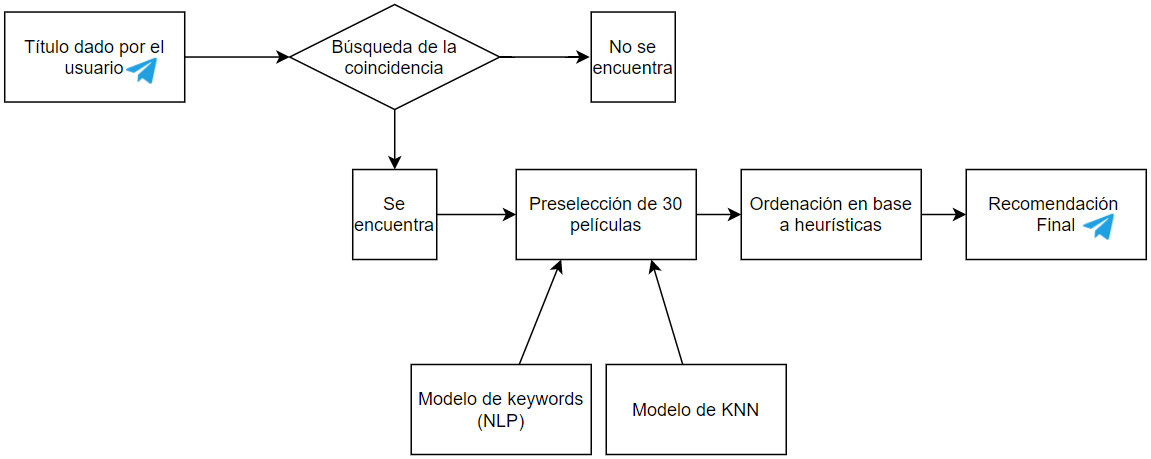
\includegraphics[width=12cm]{contenido/imagenes/FLujodattos.png}
    \caption{Flujo de la información en el sistema de recomendación.}
    \label{fig:flow}
\end{figure}


\subsection{Comparación con un sistema de filtrado colaborativo}

En la explicación de los tipos de sistemas de recomendación, ya se han enumerado las ventajas y desventajas de los dos tipos principales de sistemas. Sin embargo, una vez descrito con exactitud el sistema que hemos construido en esta memoria, consideramos oportuno el realizar una comparativa directa con otra implementación del un sistema de otro tipo; que en este caso será un sistema de filtrado colaborativo. De esta forma, se pondrá de manifiesto la aportación que realizamos al campo. Sin embargo, consideramos que nuestra aportación va más allá de una forma de crear un sistema de recomendación, por lo que en la \autoref{sec:reflexion} añadimos una pequeña reflexión sobre otras principios de diseño que hemos seguido que consideramos aportan al campo de los sistemas de recomendación.

En \cite{ilhami2014film} se realiza una implementación de un sistema de recomendación de filtrado colaborativo, aunque como puede verse en el artículo, cuentan con una cantidad de datos mucho mayor. En la \autoref{tab:compareSystems} se realiza una comparación entre el sistema propuesto en este artículo y el propuesto en este proyecto.

\begin{table}[H]
\centering
%\resizebox{0.8\textwidth}{!}{%
\begin{tabular}{p{0.3\linewidth}p{0.3\linewidth}p{0.3\linewidth}}
\hilne \textbf{Aspecto} & \textbf{Sistema de este TFE} & \textbf{Sistema propuesto en \cite{ilhami2014film}} \\ \hline 
Recomendaciones dependientes del usuario & El sistema recomienda películas independientemente del usuario que las solicita.                                                                                & Cada usuario está modelado de forma diferente, por lo que las recomendaciones sí que son únicas                                                                                                    \\
Nuevos usuarios y elementos              & Al ser independiente del usuario, la aparición de nuevos usuarios no es un problema. Los nuevos contenidos serán recomendados una vez se rellenen sus metadatos & Puede haber problemas al tener usuarios que no hayan valorado ninguna película o películas que no hayan sido recomendadas. Es el problema denominado \textit{cold start}                           \\
Posibilidad de indexación                & Podemos tener precalculadas las recomendaciones, lo cual supone un gran ahorro de tiempo a la hora de servir las recomendaciones a los usuarios                 & Tener las recomendaciones precalculadas es muy costoso, al depender del producto entre usuarios y películas.                                                                                       \\
Agnosticismo                             & El sistema recomienda las películas independientemente de la plataforma en la que se encuentran, al contrario que sistemas de Netflix o Amazon                  & El conjunto de películas utilizado no proviene de una plataforma en concreto. Sin embargo, al usar votos de usuarios, es complicado introducir una película que no esté en la plataforma de votos. \\
Implementación Real                      & El proyecto de este trabajo se ha desarrollado de una forma \textit{end to end}, de forma que se ha generado un sistema de recomendación usable                 & El sistema de recomendación creado es de laboratorio, no hay posibilidad de usarlo                                                                                                                
\end{tabular}%
%}
\caption{Comparación entre el sistema de recomendación propuesto en \cite{ilhami2014film} y en esta memoria.}
\label{tab:compareSystems}
\end{table}


\section{Reflexión}\label{sec:reflexion}

En esta sección del trabajo, queremos explicar algunas normas de diseño que se han seguido en la construcción de este sistema de recomendación. Resulta fácil pensar que este sistema difícilmente superará en términos de calidad de las recomendaciones a un sistema como el que puede tener implementado una empresa como Netflix o Amazon. Estas empresas tienen cientos de millones de usuarios y catálogos amplísimos, además de grandes equipos dedicados a crear estos sistemas de recomendación que tan lucrativos les son, pues son parte principal de su negocio. Estas empresas disponen también de información más allá de meras valoraciones de usuarios, como puede ser el tiempo de visionado de un producto antes de comprarlo o la cantidad de series que miran antes de elegir una. Datos que pueden ser muy relevantes a la hora de realizar una recomendación.\\

Consideramos que en este ambiente, somos los amantes del cine los que realmente perdemos. A la gente que le gusta el cine, que no es poca, realmente no le importa tanto dónde ver una película, sino que lo que quiere son recomendaciones significativas que le aporten valor. Es aquí donde creemos que nuestro sistema tiene uno de sus puntos fuertes. Un sistema como del de Netflix no tiene como objetivo el enriquecer tus conocimientos sobre cine, sino que por detrás existen otros intereses, menos explícitos, que son el mantenerte el máximo tiempo posible en sus plataformas, que gastes la mayor cantidad de dinero o que consumas contenidos con millones de dólares gastados en producción. Para ejemplificar esto, lanzamos una pregunta al aire: \textquestiondown cuándo fue la última vez que Netflix te recomendó una película de hace más de 20 años? Nosotros consideramos que no todo el público está orientado a consumir cine actual, y que mucha gente está dispuesta a buscar cómo consumir una película si cree que puede gustarle.\\

Además, en los últimos años, los usuarios se han vuelto cada vez más conscientes de los datos que dan a las plataformas que utilizan. Con la publicación en el año 2018 del Reglamento General de Protección de Datos, los ciudadanos de la UE vimos gratamente reforzados nuestros derechos respecto a nuestros datos personales. Plataformas como Amazon o Netflix almacenan todos los datos que les es posible, mientras que nuestra estrategia es una estrategia \textit{cero datos}, en la que intentamos no necesitar de ningún dato personal para poder realizar las recomendaciones.\\

Por tanto, dos normas de diseño que hemos mantenido en el desarrollo de este proyecto son las siguientes:

\begin{itemize}
    \item Agnosticismo: Nuestro sistema de recomendación es agnóstico respecto a la plataforma en la que se consume el contenido. Por tanto, proveemos al sistema de una interfaz propia, multiplataforma, gratuita y de acceso libre como es Telegram para que los usuarios puedan realizar consultas al sistema. El objetivo primordial es dar al usuario las recomendaciones más significativas dentro de las posibilidades de los datos disponibles, entendiendo por significativa la película que más puede gustarle, sin tener en cuenta otros intereses que los del propio usuario.
    \item Cero datos: El sistema no almacena datos de los usuarios. Con el fin de proteger la privacidad de los usuarios, el sistema no registra de forma persistida las interacciones de cada usuario con el fin de modelarlo. Esta premisa tiene la desventaja de que es un sistema que no se puede mejorar con el uso, pero si puede mejorarse a través de la realización de modelados más eficientes de las películas.
\end{itemize}



